\chapter{Integracija računalnog oblaka i razvojnog sustava}

Integracija.

\section{Probno povezivanje korištenjem demo aplikacije AWS Quick Connect}

Za početno probno povezivanje razvojnog sustava ESP32-C3 sa sustavom AWS, korištena je službena demo aplikacija \textit{Quick Connect} koja, nakon učitavanja binarne datoteke u razvojni sustav i definiranje vjerodajnica za povezivanje na Wi-Fi, putem protokola MQTT šalje informacije s uređaja u AWS \cite{quick_connect_app}. Račun za uređaj se automatski stvori te nije potrebna nikakva dodatna prijava u sam sustav. Na slici \ref{fig:aws_esp32_easy_connect} nalazi se ispis u konzoli nakon što se pokrene demo aplikacija na razvojnom sustavu. Iz slike je vidljivo postavljanje (engl. \textit{provisioning}) uređaja, kao i kreiranje certifikata za siguran prijenos podataka.

\begin{figure}[ht]
	\centering
	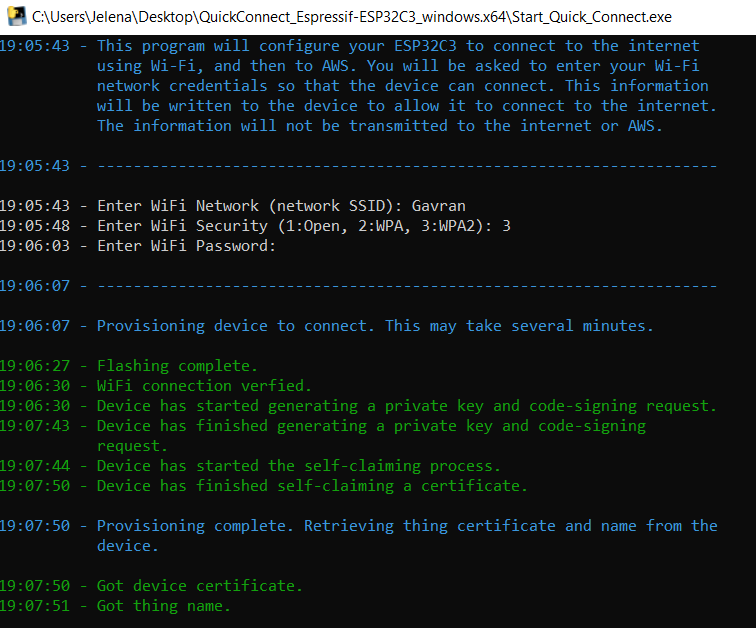
\includegraphics[scale=0.5]{imgs/aws_esp32_easy_connect}
	\caption{Ispis u konzoli pri pokretanju demo aplikacije Quick Connect}
	\label{fig:aws_esp32_easy_connect}
\end{figure}

Slika \ref{fig:esp32_easy_connect_mqtt_packages} također prikazuje ispis u konzoli, no ovaj puta sadržaj paketa koji se šalju protokolom MQTT. Podaci su prikazani u formatu JSON.

\begin{figure}[ht]
	\centering
	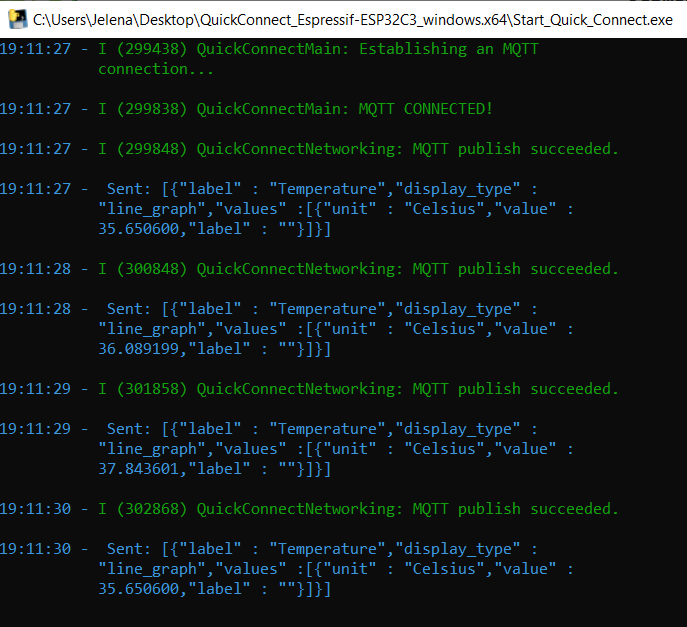
\includegraphics[scale=0.5]{imgs/esp32_easy_connect_mqtt_packages}
	\caption{Ispis slanja paketa protokolom MQTT s razvojnog sustava ESP32-C3}
	\label{fig:esp32_easy_connect_mqtt_packages}
\end{figure}

\eject